\chapter{Related Work}

\section{MOOCs}

\subsection{Overview}
MOOCs refers to massive online open courses, which is a online course platform people can access through internet connection regardless of the limit of space and time.
MOOCs is normally free, credit-less and is designed for massive people to enroll and learn.
Base on different theories, there are two kinds of MOOCs, cMOOCs and xMOOCs, which will mentioned in following section.

\subsection{cMOOCs v.s. xMOOCs}
Since ``The year of MOOCs'' \cite{pappano2012}, MOOCs have become increasingly robust and diverse in last few year.
There are many websites provide MOOCs for different group in various way.
Based on different learning theory, we classify MOOCs into cMOOCs and xMOOCs.
cMOOCs are base on the learning theory of Connectivism, this kind of MOOCs focus on network between individuals in course.
students may use any digitle platform such as Facebook, Google+, blog to make connections with other learners to create and construct knowledge.
The participants in cMOOCs act as teacher and learner at the same time as they share knoledge with each other.
Instead of being structured as an open online community of learners, xMOOCs are much more like traditional classroom environment.
xMOOCs are centered around class instroctor, instroctor usually will provide series of lecture video, where learners mainly get knowledges.
Besides, exercises, quizes, assignments are also used during the course.
Most of the popular MOOC websites in recent year are belong to xMOOCs such as Coursera, edX, Udacity, etc.

\subsection{Coursera}

\begin{figure}[H]
    \centering
    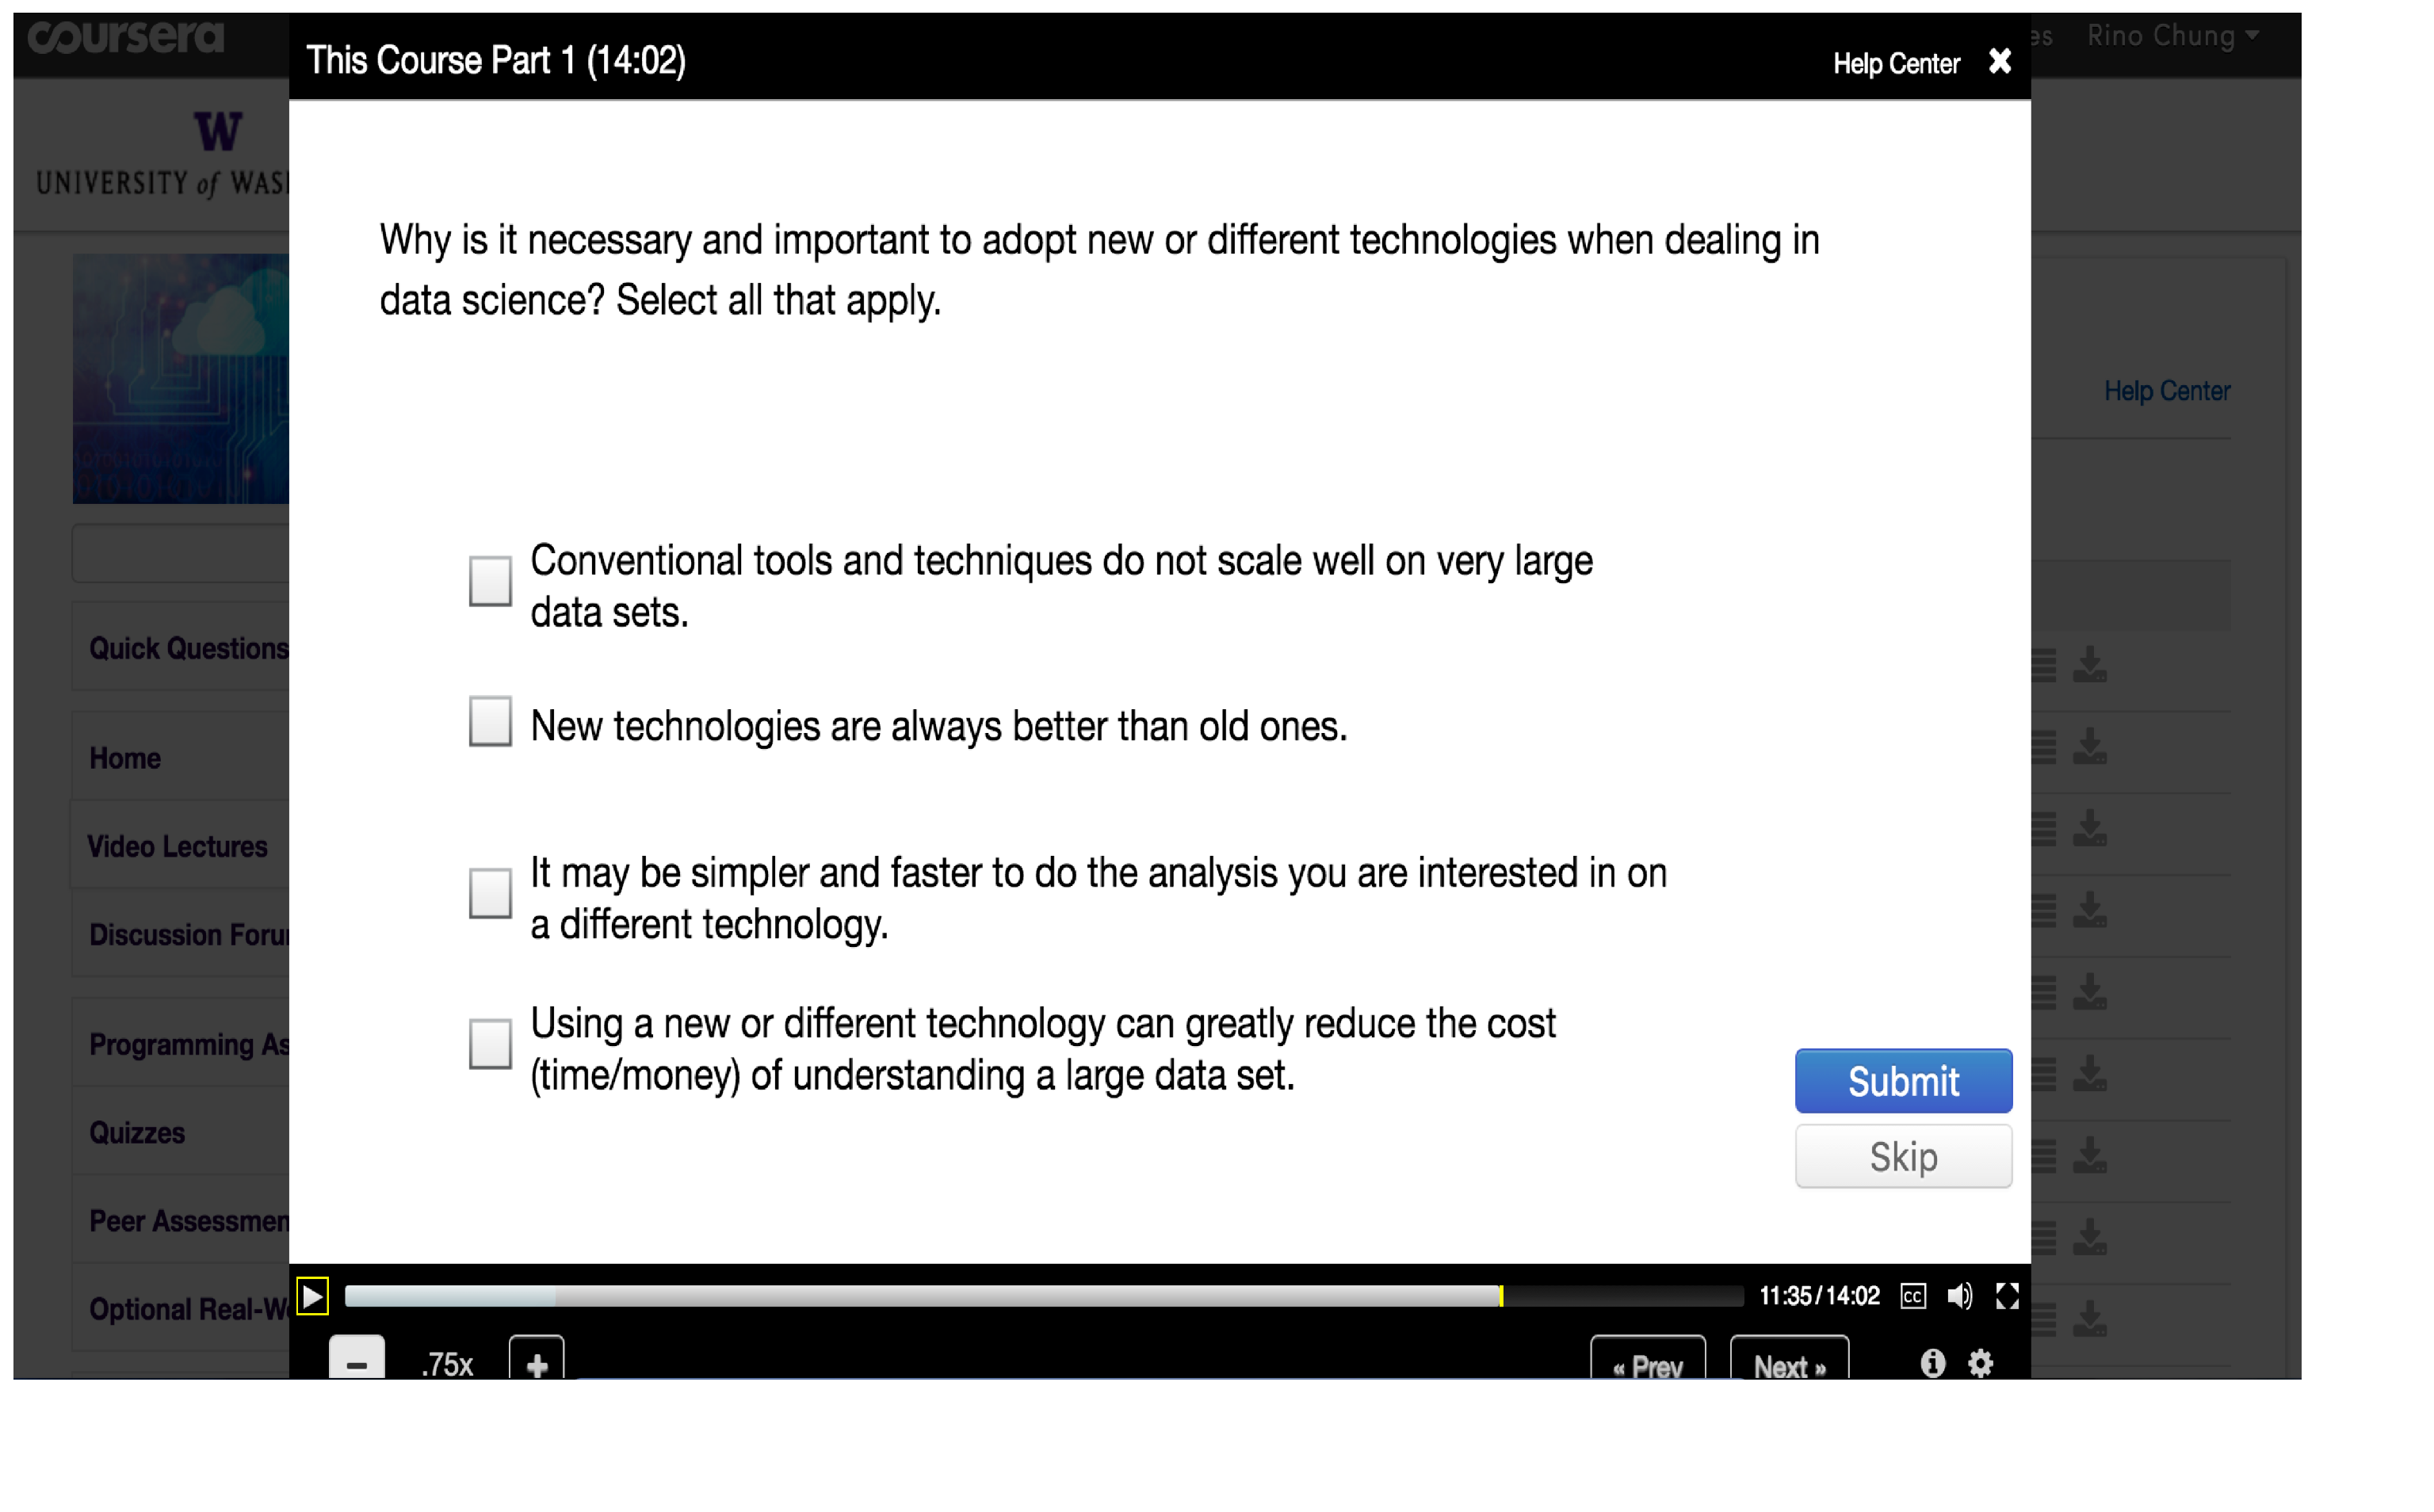
\includegraphics[width = 0.8\textwidth]{fig/coursera_pop.eps}
    \caption{Coursera pop-up question in lecture video}
    \label{fig:coursera_pop}
\end{figure}

Coursera \cite{coursera} started in 2012 founded by Stanford University. It provides courses from renowned universitise like Stanford University,  Princeton University, University of Michigan, etc.
Taking course on Course is free, learners can enroll courses that interest them at will.
Applying for hard copy certification of course, however, will charge for some money.
As a xMOOC platform, lecture videos are the major teaching material of courses with transcripts in many different language; moreover forum, exercises, assignments and other traditional xMOOC functions are also provide on Coursera.
To make sure learners focusing on the lecture video, there is a pop-up question about current video in every lecturevideo see Figure \ref{fig:coursera_pop}.
The question will let you submit three times, and if all the answers are wrong in three submission system will tell you the answer but learners can chose to continue the video without answering the question.
Coursera also has iOS, Android, and Kindle Fire apps.

\subsection{edX}
edX \cite{edx} is also a xMOOC platform, which founded by Harard University and MIT at 2012 offering high-quality courses from universities and intuitions to learners.
As a xMOOC, courses on edX center on lecture videos whit the supports like forum, exam, and other features most MOOC platform has.
Besides the majority of courses are taught in english, edX also provides some foreign language courses.
\begin{figure}[H]
    \centering
    \includegraphics[width = 0.8\textwidth]{fig/edx.eps}
    \caption{edX: a MOOC platform}
    \label{fig:coursera_pop}
\end{figure}

Similar to Coursera, edX has certificate system, which you can apply for hard copy proof when you pass the course; it will charge you certificate fee, however, the price is cheeper than Coursera.

\section{Researchs improve MOOCs learning}
hello
